As we can see from ensemble models tuning and performance we weren't able to decrease variance or bias of our predictions. So the question is: is there any possibility to reduce the prediction error?
We know from theory that:

$$\text{Error}(\mathcal{M} ) = \text{Bias}^2 + \text{Variance} + \varepsilon$$
since we know that boosting should reduce the bias and bagging (random forests) should reduce the variance, we can conclude that the error is not going to decrease, in fact we have not been able to reduce the error beyond a certain threshold that is probably the value of $\varepsilon$ in the previous formula.

  \begin{figure}[h]
    \centering
    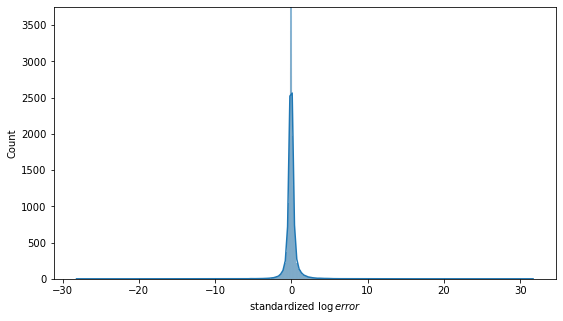
\includegraphics[width=0.8\textwidth]{img/standard_log_error_dist.png}
    \caption{Standardized distribution of the log error}
  \end{figure}

The distribution of data confirms this thesis: standardizing the distribution of the $\log error$ we get a normal distribution with mean 0 and variance 1, but with extremely long tails (data goes from $-30$ to $30$). The fact is that predict an error $e$ such that $|e| > 4$ in a standard normal distribution is nearly impossible, we have to conclude that those tails include many outliers (or data from another kind of distribution) and that the model is not able to predict them.

The problem is that houses with wrong error prediction are not really different from other ones. If we assume that most of the errors have been made by humans\footnote{Often in large dataset problems come from data input. In this case we have a confirm from this conversation (\url{https://www.kaggle.com/competitions/zillow-prize-1/discussion/36752}), where we read that it's more likely that when Zestimate gets a high error in reality it did well, while the sell price in the database was inserted with an error.} it is not a surprise to see that errors are most incident where there are more data (imagine who inputs a lot of data has an high chance to input something wrong) and we still get that the error due to data input is not predictable.

The conclusions of this analysis have led us to this point, this does not mean that the work to predict the log error is finished, here is a list of possible steps from which to start for further investigations:

\begin{itemize}
  \item perhaps data cleaning was not adeguate, try removing data in a different way;
  \item we found that predict outliers is nearly impossible, we could drop them or create a specialized model for outliers;
  \item try focus on new features based on the features importance we got from the analysis, it could be that a ratio $taxes assessed \over sqare feets$ have an impact on prediction;
  \item apply different transformations on data to change their distribution.
\end{itemize}
